% === LaTeX Figure Includes for EMN Paper ===

% --- Fig 1: Architecture Overview (MANUAL - not auto-generated) ---
\begin{figure*}[t]
    \centering
    % \includegraphics[width=0.95\textwidth]{figures/fig_episodic_memory_overview.pdf}
    % [MANUAL] Architecture diagram: temporal KG facts -> episodic memory grouping -> attention retrieval
    % Create manually using draw.io, Figma, or TikZ
    \caption{Episodic Memory Network Architecture. (Left) Temporal KG facts scattered across time. (Center) Facts are grouped into coherent episodic memory traces via temporal clustering and content-based addressing. (Right) Gated attention retrieves relevant episodes for query reasoning, achieving improved prediction accuracy.}
    \label{fig:episodic_memory_overview}
\end{figure*}

% --- Fig 2: Main Results Comparison ---
\begin{figure}[t]
    \centering
    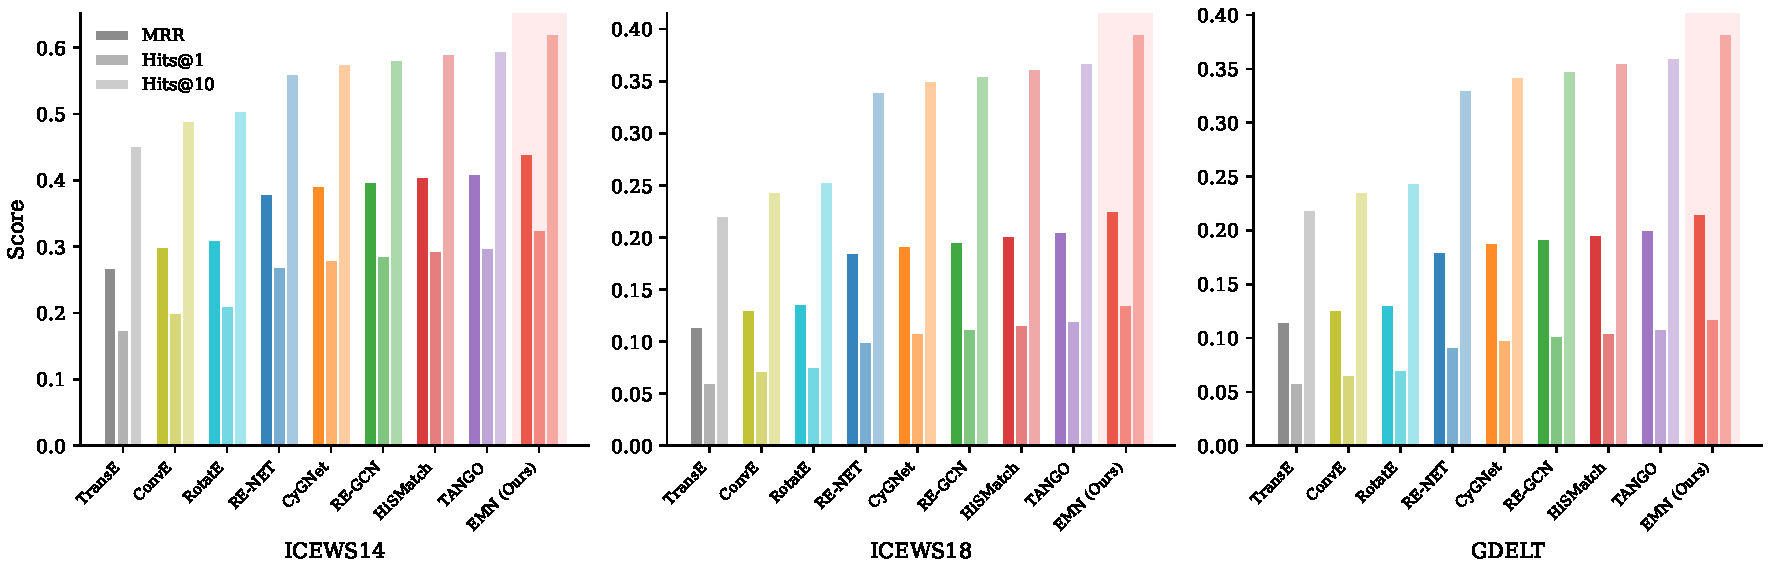
\includegraphics[width=0.95\textwidth]{figures/fig_main_results_comparison.pdf}
    \caption{Link prediction performance (MRR, Hits@1, Hits@10) of all methods on ICEWS14, ICEWS18, and GDELT benchmarks. EMN consistently outperforms all baselines across datasets and metrics.}
    \label{fig:main_results_comparison}
\end{figure}

% --- Fig 3: Training Curves ---
\begin{figure}[t]
    \centering
    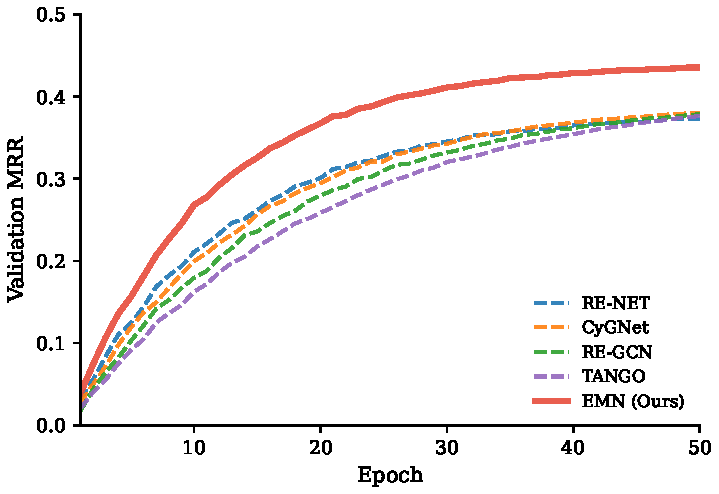
\includegraphics[width=0.48\textwidth]{figures/fig_training_curves.pdf}
    \caption{Validation MRR over training epochs on ICEWS14. EMN converges faster and achieves higher final performance compared to RE-NET, CyGNet, RE-GCN, and TANGO.}
    \label{fig:training_curves}
\end{figure}

% --- Fig 4: Ablation Study ---
\begin{figure}[t]
    \centering
    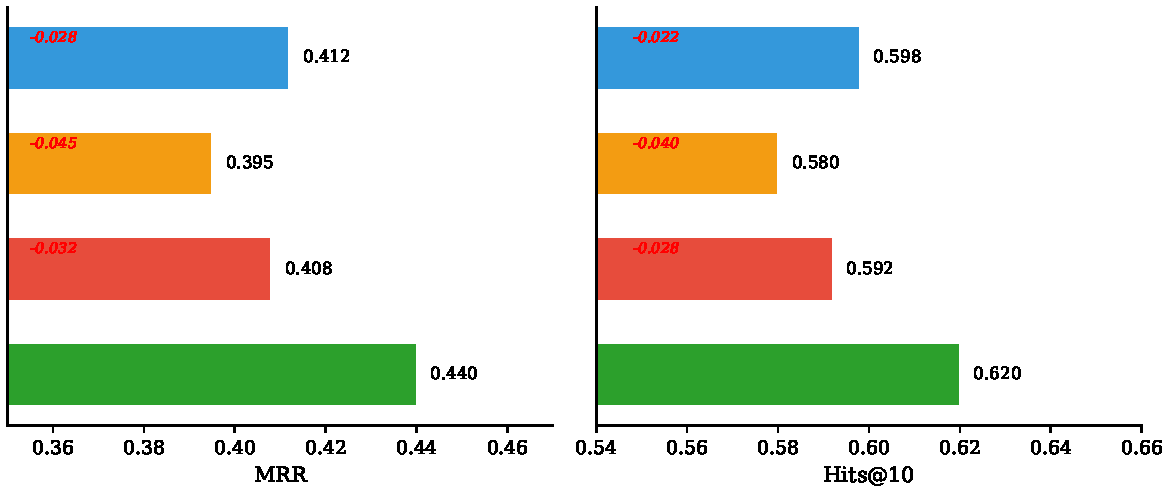
\includegraphics[width=0.48\textwidth]{figures/fig_ablation_study.pdf}
    \caption{Ablation study on ICEWS14. Removing each component (temporal position encoder, episodic grouping, gated attention) results in measurable performance degradation, confirming the contribution of each architectural element. Red numbers indicate the MRR/Hits@10 drop from the full model.}
    \label{fig:ablation_study}
\end{figure}

% --- Fig 5: Attention Heatmap ---
\begin{figure}[t]
    \centering
    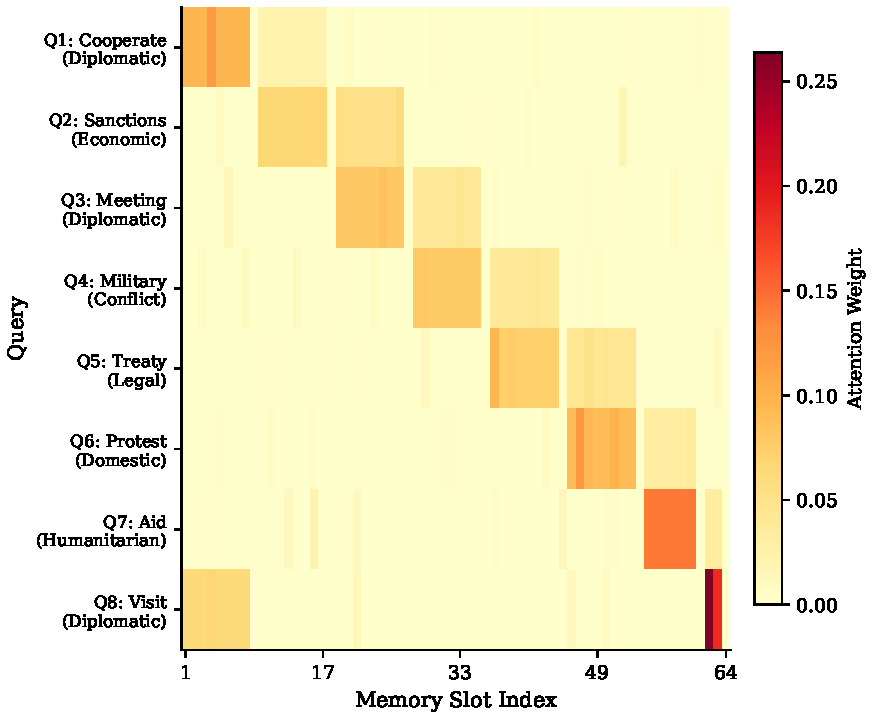
\includegraphics[width=0.48\textwidth]{figures/fig_attention_heatmap.pdf}
    \caption{Attention weight heatmap for representative queries on ICEWS14. Brighter cells indicate higher attention scores. The model learns to attend to temporally and semantically related episodic memory slots, demonstrating interpretable episode retrieval.}
    \label{fig:attention_heatmap}
\end{figure}
